\subsection{Service Clients}\label{p:client}

This problem is designed to introduce the client-service structure. For this question you will be
using our implemented service and writing your own client to create a slightly different single
flower then before. See Figure~\ref{fig:2} for what the flower should look like.

The work for this problem should be done in file \texttt{client.py}.

\begin{figure}[h]
  \centering
  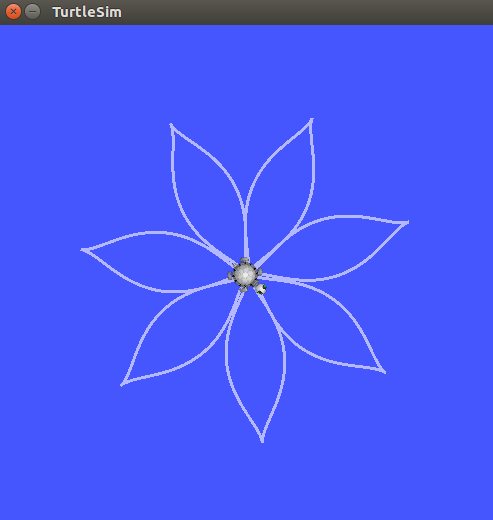
\includegraphics[width=150pt]{figures/p1/problem3.png}
  \caption{For Problem~\ref{p:client}. Service Clients}
  \label{fig:2}
\end{figure}

In \texttt{draw\_flower}:
\begin{enumerate}[(a)]
  \item Initialize your node with the name \texttt{drawing\_turtle}.
  \item Wait for the service \texttt{draw}.

  \item Get a service handle for the draw service. Check \texttt{srv/Draw.srv} and \texttt{rospy}
    documentation for more information.

  \item Make a publisher that publishes to \texttt{/turtle1/cmd\_vel} with type \texttt{Twist} and
    queue size of 10
  \item Make a 5Hz \texttt{Rate}.

  \item Loop, and:
    \begin{enumerate}[i.]
      \item Use the draw service to get the velocity message to publish. Look at \texttt{srv/Draw.srv}
        to determine the parameters and appropriate return name.
      \item Sleep for the previously created rate.
    \end{enumerate}
\end{enumerate}

In the main script:
\begin{enumerate}[(a)]
  \item Call your function to draw the flower!
\end{enumerate}

In \texttt{client.launch}:
\begin{enumerate}[(a)]
  \item Launch the turtlesim node.
  \item Launch the \texttt{draw\_service} node.
  \item  Launch the \texttt{draw\_flower} node.
\end{enumerate}
